\chapter{システムの設計・実装}
\label{chap:implementation}

% 本章では、\ref{chap:network_transmission}章で提示した、

\section{UoIP} % UHD over IP

\section{システム構成}



\section{ソフトウェアによる実装}

本実装では、汎用的なデスクトップコンピュター、Intel 10Gbps NIC、

\begin{figure}[htbp]
    \begin{center}
        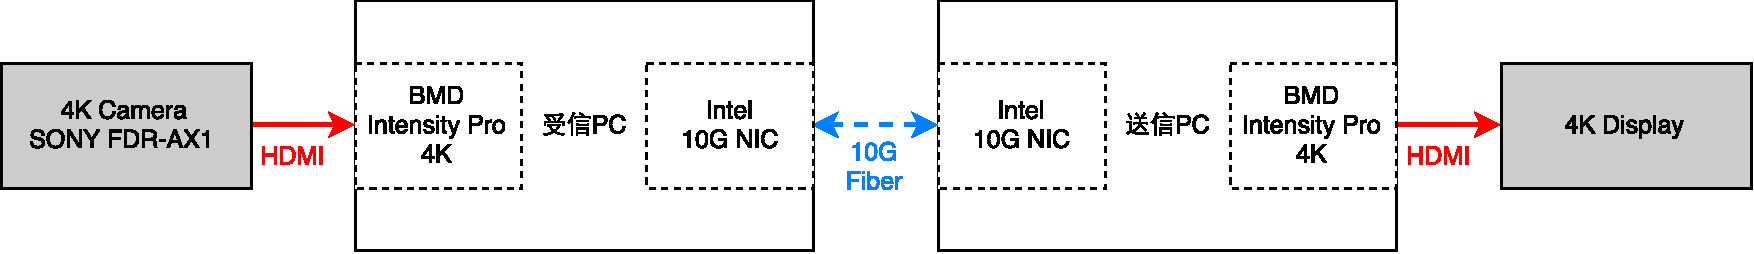
\includegraphics[bb=0 0 841 121,width=15.5cm]{img/software-implement-flow.pdf}
    \end{center}
    \caption{ソフトウェアによる実装の構成}
    \label{fig:software-implement-flow}
\end{figure}

\begin{figure}[htbp]
    \begin{center}
        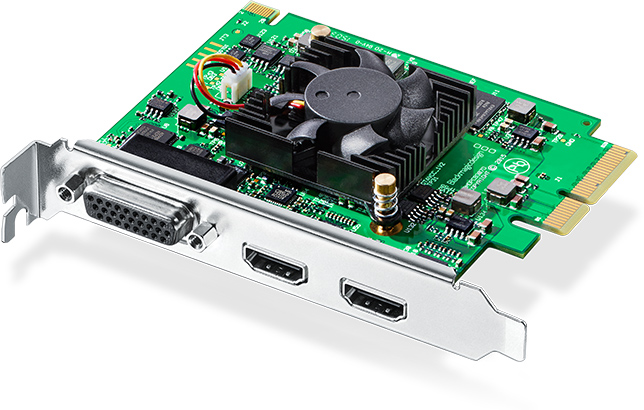
\includegraphics[bb=0 0 644 410,width=5cm]{img/bmd-intensity-pro-4k.jpg}
    \end{center}
    \caption{Blackmagic Design Intensity Pro 4K キャプチャーボード}
    \label{fig:ted-4k-fmc-card}
\end{figure}

\section{ハードウェアによる実装}

\subsection{FPGAの回路設計}

Axi4-Stream、tuser
図\ref{fig:fpga-video-ethernet-diagram}
図\ref{fig:fpga-ethernet-video-diagram}

本実装では、Xilinxの 10 Gigabit Ethernet Subsystem、及び、Video Processing Subsystemを用いた。

\begin{figure}[htbp]
    \begin{center}
        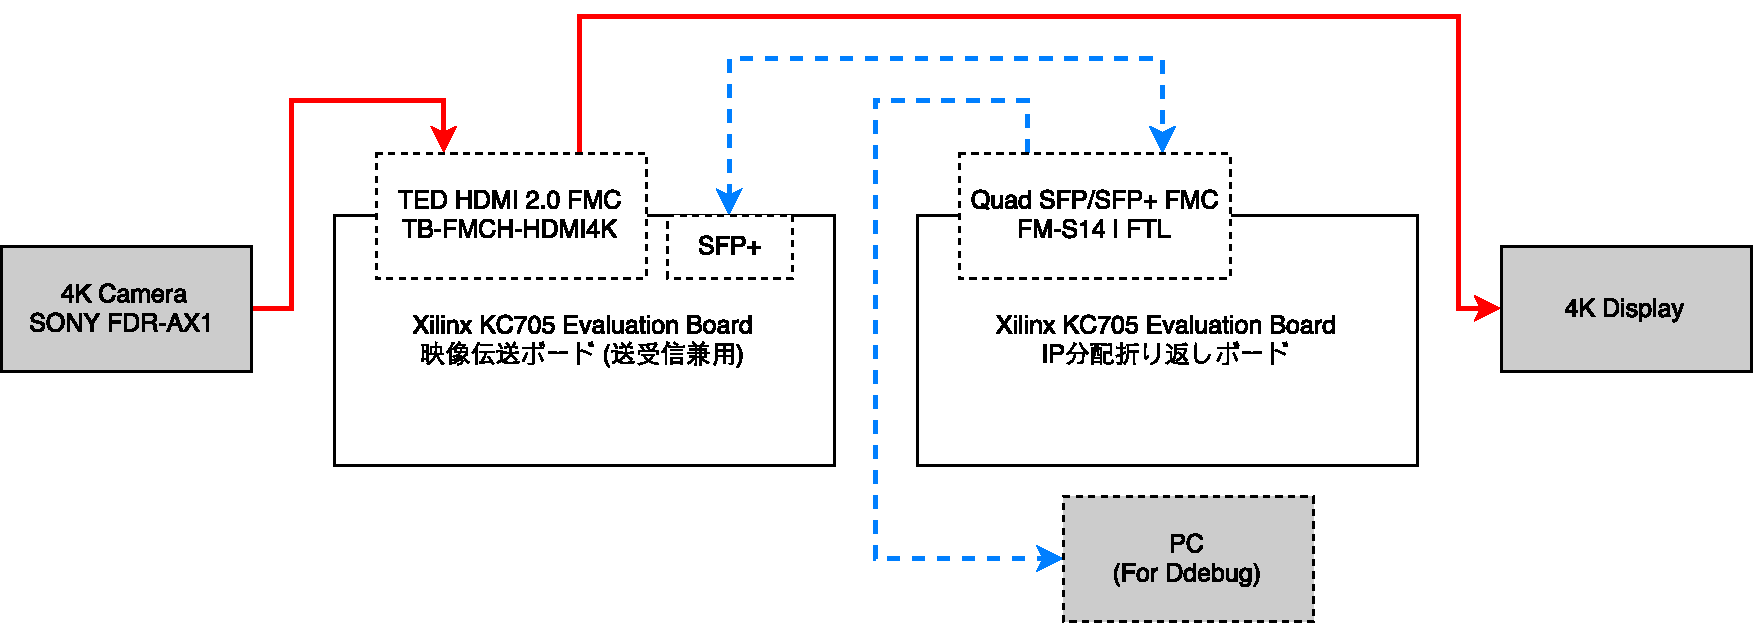
\includegraphics[bb=0 0 841 299,width=15.5cm]{img/fpga-implement-flow.pdf}
    \end{center}
    \caption{ハードウェアによる実装の構成}
    \label{fig:fpga-implement-flow}
\end{figure}

% 本実装の概要を、図\ref{fig:fpga-implement-flow}に示す。

\begin{figure}[htbp]
    \begin{center}
        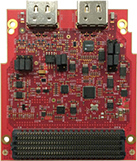
\includegraphics[bb=0 0 137 161,width=4cm]{img/ted-4k-fmc-card.jpg}
    \end{center}
    \caption{TED HDMI 2.0 FMCカード (TB-FMCH-HDMI4K)}
    \label{fig:ted-4k-fmc-card}
\end{figure}

% 10 Gigabit Ethernet Subsystemの挙動に空いては、Xilinx PG157\cite{xilinx-pg157}を参照されたし。
% \cite{xilinx-pg235}
% \cite{xilinx-pg236}

\begin{table}[htbp]
  \caption{HDMI RX SubsystemのAxi4-Streamインターフェース \cite{xilinx-pg236}より抜粋}
  \label{tb:pg236-vout-axi4-stream}
  \begin{center}
  \begin{tabular}{l|c|c|l}
    \hline
    Name   & Direction & Width     & Description \\\hline\hline
    tdata  & Output    & 3*BPC*PPC & Data \\\hline
    tlast  & Output    & 1         & End of line \\\hline
    tready & Input     & 1         & Ready \\\hline
    tuser  & Output    & 1         & Start of frame \\\hline
    tvalid & Output    & 1         & Valid \\\hline
  \end{tabular}\end{center}
\end{table}

\begin{table}[htbp]
  \caption{HDMI TX SubsystemのAxi4-Streamインターフェース \cite{xilinx-pg235}より抜粋}
  \label{tb:pg236-vin-axi4-stream}
  \begin{center}
  \begin{tabular}{l|c|c|l}
    \hline
    Name   & Direction & Width     & Description \\\hline\hline
    tdata  & Input     & 3*BPC*PPC & Data \\\hline
    tlast  & Input     & 1         & End of line \\\hline
    tready & Output    & 1         & Ready \\\hline
    tuser  & Input     & 1         & Start of frame \\\hline
    tvalid & Input     & 1         & Valid \\\hline
  \end{tabular}\end{center}
\end{table}

\begin{figure}[htbp]
    \begin{center}
        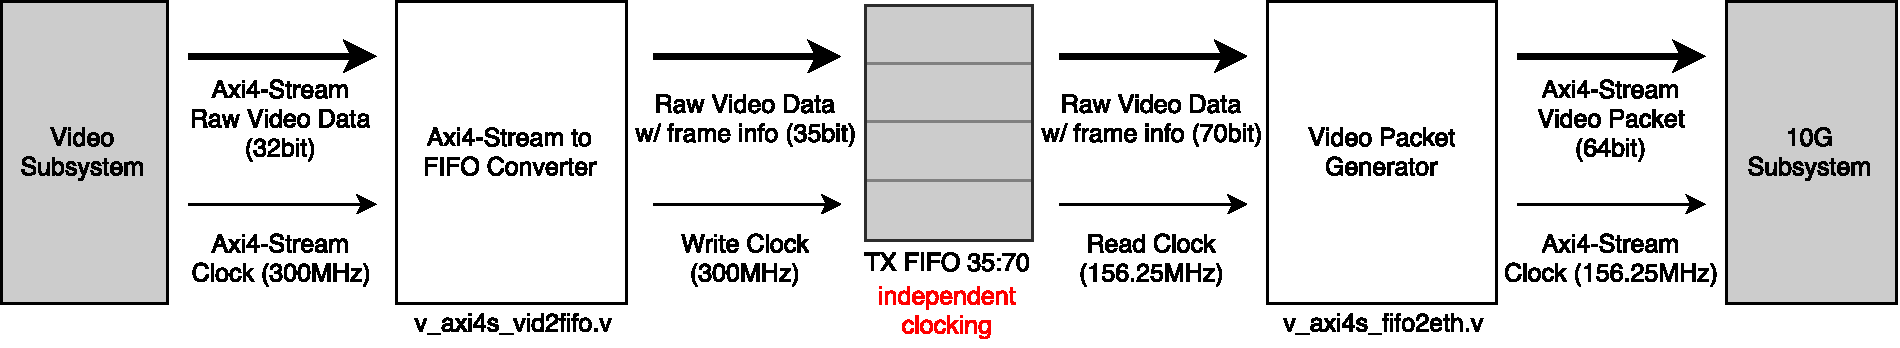
\includegraphics[bb=0 0 911 166,width=15.5cm]{img/fpga-video-ethernet-diagram.pdf}
    \end{center}
    \caption{Video Stream to Ethernet Packet Subsystem Diagram}
    \label{fig:fpga-video-ethernet-diagram}
\end{figure}

\begin{figure}[htbp]
    \begin{center}
        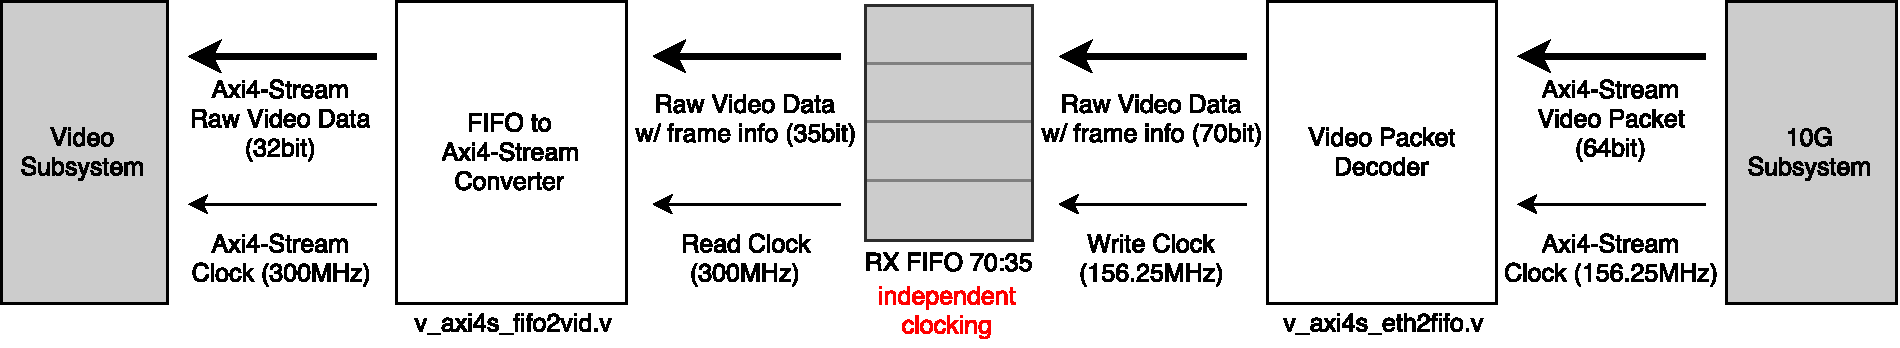
\includegraphics[bb=0 0 911 166,width=15.5cm]{img/fpga-ethernet-video-diagram.pdf}
    \end{center}
    \caption{Ethernet Packet to Video Stream Subsystem Diagram}
    \label{fig:fpga-ethernet-video-diagram}
\end{figure}

% 図\ref{fig:fpga-video-packet}に、本実装で用いたパケット構造を示す。



\begin{figure}[htbp]
    \begin{center}
        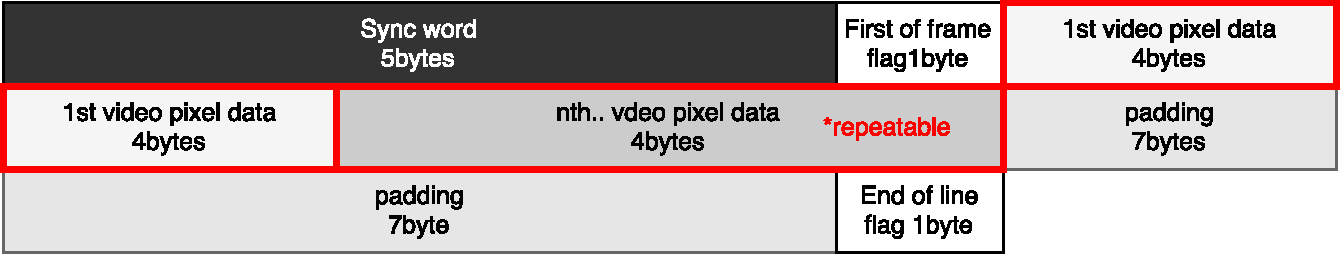
\includegraphics[bb=0 0 643 122,width=15.5cm]{img/fpga-video-packet.pdf}
    \end{center}
    \caption{Video Packet Structure}
    \label{fig:fpga-video-packet}
\end{figure}

ビデオデータより前の区間が6byte、Ethernetパケットを構築、64bitごとに生成するため、tcpのペイロード部分が区切りが


\begin{figure}[htbp]
    \begin{center}
        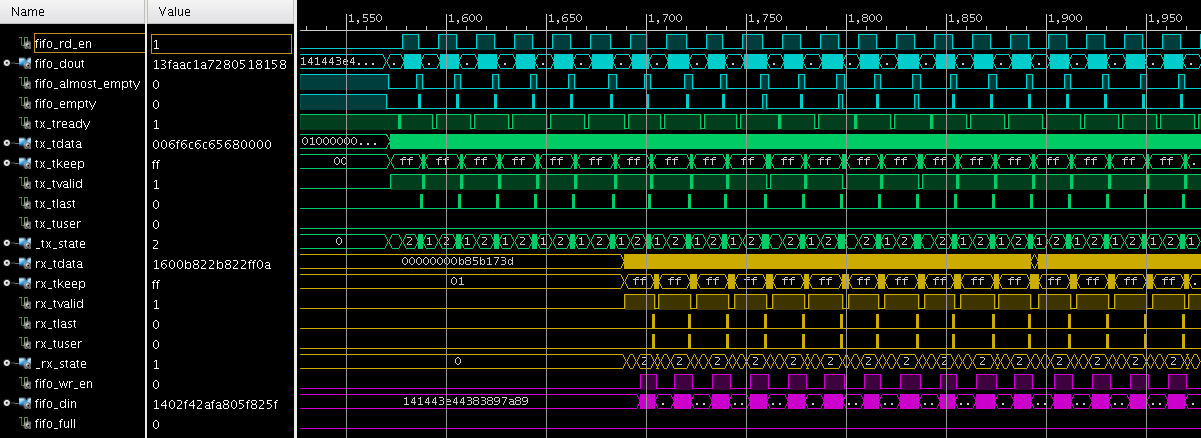
\includegraphics[bb=0 0 1201 438,width=15.5cm]{img/fpga-ila-fifo-to-eth.png}
    \end{center}
    \caption{Video Packet Structure}
    \label{fig:fpga-ila-fifo-to-eth}
\end{figure}

\begin{figure}[htbp]
    \begin{center}
        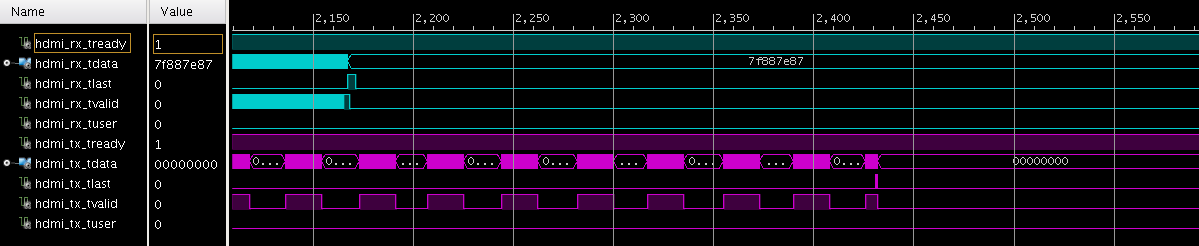
\includegraphics[bb=0 0 1199 246,width=15.5cm]{img/fpga-ila-hdmi.png}
    \end{center}
    \caption{Video Packet Structure}
    \label{fig:fpga-ila-hdmi}
\end{figure}

\begin{figure}[htbp]
    \begin{center}
        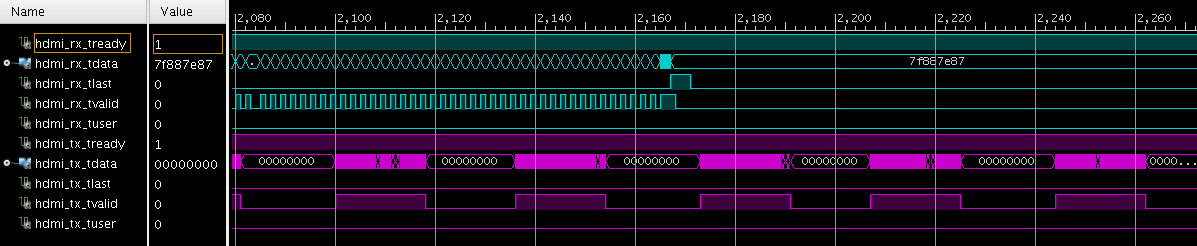
\includegraphics[bb=0 0 1197 246,width=15.5cm]{img/fpga-ila-hdmi-x2.png}
    \end{center}
    \caption{Video Packet Structure}
    \label{fig:fpga-ila-hdmi-x2}
\end{figure}
